\chapter{Software architecture}
\label{SoftwareArchitecture}

\begin{flushright}{\slshape    
Interaction is an iterative process of listening, thinking, \\
and speaking between two or more actors.} \\ \medskip
    --- Chris Crawford, game designer
\end{flushright}

\marginpar{Parts of this chapter have previously appeared in \cite{Niezen2010} and \cite{Niezen2012}}

Existing architectural patterns for software like the \ac{MVC} model, Document-View and Presentation-Abstract-Control are considered to be inadequate when trying to design software architectures in the ubiquitous computing domain. Ubiquitous computing needs new kinds of mechanisms to meet the flexibility needed to change the purpose, functionality, quality and context of a software system \cite{Niemela2004}.\marginpar{\ac{MVC} was first mentioned in Section \ref{InteractionModels}.}

In this chapter the software architecture used in the three design iterations is described in more detail. It is quite a short chapter, as most of the software architecture issues have already been discussed in the three design iteration implementations in Sections \ref{D1Implementation}, \ref{D2Implementation} and \ref{D3Implementation}. However, we consider it important that the final software architecture design has its own dedicated chapter, so that it can act as a reference design for future implementations.

We first look at some characteristics of ubicomp middleware, followed by a discussion of the publish/subscribe paradigm and the blackboard architectural pattern. We then look at the \ac{MOM} implementation used within the \ac{SOFIA} project, called \ac{SSAP}. The rest of the chapter is dedicated to the two main implementations of the software architecture as used within the \ac{SOFIA} project -- Smart-M3 and ADK-SIB. These implementations are interoperable with one another through the use of \ac{SSAP}.


\section{Characteristics of ubicomp middleware}

There are a number of characteristics, or quality attributes, that are specific to middleware for ubiquitous computing, as defined by Niemel\"a and Vaskivuo \cite{Niemela2004}:

\begin{itemize}
	\item Interoperability
	\item Scalability 
	\item Reusability
	\item Maintainability
	\item Extensibility
	\item Portability
	\item Adaptability
	\item Survivability
	\item Agility
	\item Fidelity
\end{itemize} 

Interoperability is defined as the ability for software applications written in different programming languages, running on different platforms with different operating systems, to communicate and interaction with one another over different networks. Scalability is the ability of the system to handle larger numbers of smart objects. Re\-us\-a\-bility, maintainability and extensibility are characteristics that consider the evolution of software systems. Portability and adaptability are important characteristics for software that has to work in a heterogenous system of devices and networks. Survivability is the ability of a system to timely deliver essential services in the face of attack, failure or accident. Agility is the sensitivity to changes in resource availability. Fidelity is defined to mean to degree to which data presented on a client matches the reference copy at the server.

We focused on a subset of these attributes while working on the software architecture, including interoperability, reusability, maintainability and extensibility. Interoperability was achieved by adhering to the \ac{SSAP} specification, as described in more detail in Section \ref{ssap}. Using ontologies and other Semantic web technologies helped us to improve reusability, while elements of maintainability were tested using the Cognitive Dimensions framework, described in more detail in Chapter \ref{Evaluation}. Extensibility was achieved by modelling devices and their capabilities in such a way that other devices could easily be added to the system.
\marginpar{Potential scalability was tested by evaluating the performance of the software architecture, as described in Section \ref{performance}.}
% \subsection{Context}
% 
% Context is information that can be used to characterise the situation of an entity, where an entity can be a person, place, or physical or computational object \cite{Gu2004}. Context awareness is the capability of ubiquitous computing middleware to handle unpredictable changes \cite{Niemela2004}. Application-aware adaption is part of context awareness, defined to mean to collaboration between the system infrastructure and the individual applications on the devices.


\section{Publish/subscribe paradigm and the blackboard architectural pattern}
\label{pubsubblackboard}
In publish/subscribe systems, subscribers register their interest in a specific event, and are notified when this event occurs after a publisher publishes the event. The strength of the publish/subscribe par\-a\-digm is that entities are decoupled in time, space and synchronisation \cite{Eugster2003}. Space decoupling means that the interacting entities do not need to be aware of each other. Time decoupling means that the entities do not need to participate in the interaction at the same time. Synchronisation decoupling means that subscribers can asynchronously be notified when an event occurs. Removing synchronisation dependencies between entities increases scalability.

There are three variants of publish/subscribe systems:

\begin{itemize}
	\item Topic-based -- Entities subscribe to individual topics, usually with some form of hierarchical addressing to organise the topics
	\item Content-based -- Consumers subscribe to selective events by specifying filters, using some kind of subscription language
	\item Type-based -- Events are filtered according to their type
\end{itemize}

In the \ac{SOFIA} project, \acp{KP} communicate with a message broker using the blackboard architectural pattern, where the message broker uses a triple store as a common knowledge base. Communication between \acp{KP} occurs through the insertion and removal of triples into or from the triple store.  Given a set of smart devices, the blackboard may be used to share information between these devices, rather than have the devices explicitly send messages to one another. If this information is also stored according to some ontological representation, it becomes possible to share information between devices that do not share the same representation model, and focus on the semantics of that information \cite{Oliver2008}. The \ac{SIB} is the information store of the smart space, and contains the blackboard, ontologies, reasoner and required service interfaces for the \acp{KP} or agents.

This blackboard approach is complemented by a publish/subscribe component, that allows \acp{KP} to subscribe to specific triples in the triple store. The \acp{KP} are then notified when these triples are added, removed or updated in the triple store. Communication between the \acp{KP} and \ac{SIB} occurs using \ac{SSAP}, which is the focus of the next section.

%Publish/Subscribe mechanism (http://en.wikipedia.org/wiki/Publish/subscribe , distributed event handling system, Observer pattern as a subset that can be compared with MVC pattern, see) vs polling mechanism


%SISS2010 start

%\section{Architectural patterns for pervasive computing}

%The approach used in \ac{SOFIA} is to make use of a blackboard architectural pattern to enable cross-domain interoperability. 



%SOFIA takes the agent, blackboard and publish/subscribe concepts and re-implements them in a lightweight manner suitable for small, mobile devices. These agents, which are termed \acp{KP} can operate autonomously and anonymously by sharing information through blackboard spaces (see Figure \ref{blackboard}). T

%SISS2010 end


\section{Smart Space Access Protocol (SSAP)}
\label{ssap}

\ac{MOM} is used to send messages between components in a distributed system. Commercial options include \ac{JMS}, \ac{MSMQ} and IBM's WebSphere framework.  \ac{AMQP} is an emerging standard, of which RabbitMQ\footnote{http://www.rabbitmq.com/} is a popular implementation. ZeroMQ\footnote{http://www.zeromq.org/}, also written as \O MQ , was created to be simpler and faster than the \ac{AMQP} standard, and does not require a dedicated message broker. Other message protocols include \ac{XMPP}, \ac{MQTT} and \ac{STOMP}.\marginpar{\ac{XMPP} is an \ac{IETF} standard.}

In the \ac{SOFIA} software architecture, \acp{KP} communicate with the \ac{SIB} through \ac{SSAP} messages \cite{Honkola2010} over TCP/IP. \ac{SSAP} consists of a number of operations to insert, update and subscribe to information in the \ac{SIB}. These operations are encoded using \ac{XML}.

For operations initiated by a \ac{KP}, the \ac{KP} sends a request message and the \ac{SIB} responds with a corresponding confirmation message. For \ac{SIB} initiated operations, the \ac{SIB} sends an indication message and the \ac{KP} does not respond. Every session must start with a join operation, and a leave operation ends a session.

To insert information into the triple store, an insert operation is used by the \ac{KP}, where the triples are encoded in RDF/XML.  A \ac{SIB} confirmation message indicate whether the operation was successful or not. Similarly, a remove operation is used to remove information from the triple store. An update operation removes information from the triple store and inserts new information as an atomic operation.

To query the triple store, a template consisting of a list of triples is used, where each triple may have a wildcard as its subject, predicate or object. The result of the query is a list of all triples that match the template.

A subscribe operation creates a persistent query that is stored in the \ac{SIB} and is re-evaluated automatically after each change to the contents of the triple store. An unsubscribe operation will terminate a persistent query.

\ac{SSAP} is supported by both the \ac{SIB} implementations used in our work, such that software developed for the one implementation is also interoperable with the other implementation. We now focus in more detail on these two implementations: Smart-M3 and ADK-SIB.\marginpar{The Smart-M3 implementation was used during the first design iteration, while the ADK-SIB implementation was used during the second and third design iteration.}


%SeNAmI start
\section{Smart-M3 architecture}
\label{m3}
The M3 (multi-device, multi-vendor, multi-domain) architecture is an interoperability platform based on a blackboard architectural model that implements the ideas of space-based computing \cite{Honkola2010}. It consists of two main components: a \ac{SIB} that acts as a common, semantic-oriented store of information and device capabilities, and \acp{KP}, virtual and physical smart objects that interact with one another through the \ac{SIB}. Various \ac{SIB} implementations exist that conform to the M3 specification of which Smart-M3, developed by Nokia, was the first open source reference implementation released in 2009\footnote{http://sourceforge.net/projects/smart-m3/}. \ac{RIBS}, developed by VTT, is a C-based implementation of M3 targeted for devices with low processing power, but requires a large amount of memory \cite{Etelapera2011}.  


\section{ADK-SIB}

The \ac{SIB} implementation used during the second and the third design iteration is called ADK-SIB (Application Development Kit SIB) and was developed within the \ac{SOFIA} project. The ADK-SIB is a Jena-based\footnote{http://jena.sourceforge.net/} \ac{SIB} written in Java and runs on the \ac{OSGi} framework.

Reasoning in the standard ADK-SIB is implemented using the Jena Ontology API, but only basic reasoning with symmetric properties and transitive properties is supported. Our main contribution to improve the ADK-SIB implementation was to implement support for OWL 2 RL/RDF Rules reasoning, as well as \ac{SPIN} rules using the TopBraid \ac{SPIN} API\footnote{http://topbraid.org/spin/api/}.\marginpar{The ADK-SIB and SPIN API was first mentioned in Section \ref{adk-sib}.}

When the \ac{SIB} starts up, we first load the ontology, written in \ac{OWL} 2, from a specified web address into our \emph{asserted} model. We then load the OWL 2 RL specification, specified as \ac{SPIN} rules, from another \ac{OWL} file. We also load any custom \ac{SPIN} functions into a third model. We then build a union model of the three models and store all the asserted triples in a hashmap to improve lookup efficiency. Finally the TopSPIN reasoning engine performs inferencing across the union model, and all the inferences are stored in the \emph{inferred} model.

Whenever a new triple is added, removed or updated, the inferred model is cleared and inferencing is performed using the reasoning engine. This means that no inferencing needs to be performed when a query is run. 

\begin{figure}[bth]
	\centering
	\centerline{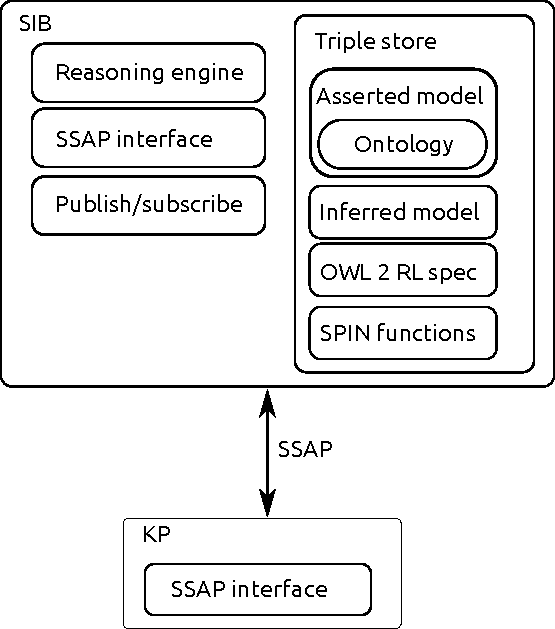
\includegraphics[width=250px]{swarch}}
	\caption{Our software architecture}
	\label{swarch}
\end{figure}

The final software architecture is shown in Figure \ref{swarch}. The system performance of the software architecture was evaluated during the Smart Home pilot of the second design iteration, and this evaluation is described in the next chapter. A validation of the entire system, including the ontology, using the Cognitive Dimensions framework is also described.


% (the following was mentioned in DesignIteration2)
% With \ac{SPIN}, rules are expressed in \ac{SPARQL}, the W3C recommended \ac{RDF} query language, which allows for the creation of new individuals using CONSTRUCT queries. OWL (Web Ontology Language) inferences for the OWL 2 RL (OWL 2 Rule Language) profile were executed by using SPIN rules\footnote{ http://topbraid.org/spin/owlrl-all}. OWL 2 RL is a syntactic subset of OWL 2 that is amenable to implementation using rule-based technologies. According to the OWL 2 RL W3C page\footnote{http://www.w3.org/TR/owl2-profiles/\#OWL\_2\_RL} the OWL 2 RL profile is aimed at applications that require scalable reasoning without sacrificing too much expressive power.


%(\texttt{OWL\_DL\_MEM\_TRANS\_INF})

% A command-line tool called \texttt{ssls}\footnote{Available from \texttt{http://sourceforge.net/projects/ssls/}} was used to view information in the smart space.

%SeNAmI end

% The SOFIA IOP is based on a blackboard architectural model that implements the ideas of space-based computing \cite{Honkola2010}. It consists of two main components: a SIB (Semantic Information Broker) that acts as a common, semantic-oriented store of information and device capabilities, and KPs (Knowledge Processors), virtual and physical smart objects that interact with one another through the SIB. Various SIB implementations exist that conform to the M3 specification, of which Smart-M3 was the first open source reference implementation released in 2009\footnote{http://sourceforge.net/projects/smart-m3/}. RIBS (RDF Information Base System) is a C-based implementation of M3 targeted for devices with low processing power, but requires a high amount of memory \cite{Etelapera2011}.  The SIB implementation used in the pilot is called ADK-SIB (Application Development Kit SIB) and was developed within the SOFIA project. 
% 
% The ADK-SIB is a Jena-based\footnote{http://jena.sourceforge.net/} SIB written in Java and runs on the OSGi (Open Services Gateway initiative) framework. Some modifications were made to the standard ADK-SIB provided by the SOFIA project, such as reasoning support added with the TopBraid SPIN API 1.2.0\footnote{http://topbraid.org/spin/api/}. 

